% THIS IS SIGPROC-SP.TEX - VERSION 3.1
% WORKS WITH V3.2SP OF ACM_PROC_ARTICLE-SP.CLS
% APRIL 2009
%
% It is an example file showing how to use the 'acm_proc_article-sp.cls' V3.2SP
% LaTeX2e document class file for Conference Proceedings submissions.
% ----------------------------------------------------------------------------------------------------------------
% This .tex file (and associated .cls V3.2SP) *DOES NOT* produce:
%       1) The Permission Statement
%       2) The Conference (location) Info information
%       3) The Copyright Line with ACM data
%       4) Page numbering
% ---------------------------------------------------------------------------------------------------------------
% It is an example which *does* use the .bib file (from which the .bbl file
% is produced).
% REMEMBER HOWEVER: After having produced the .bbl file,
% and prior to final submission,
% you need to 'insert'  your .bbl file into your source .tex file so as to provide
% ONE 'self-contained' source file.
%
% Questions regarding SIGS should be sent to
% Adrienne Griscti ---> griscti@acm.org
%
% Questions/suggestions regarding the guidelines, .tex and .cls files, etc. to
% Gerald Murray ---> murray@hq.acm.org
%
% For tracking purposes - this is V3.1SP - APRIL 2009

% require the `acm_proc_article-sp.cls` file.
\documentclass{acm_proc_article-sp}

\usepackage{url}
\usepackage{paralist}
\usepackage{graphicx}
\usepackage{subfigure}

\begin{document}

\title{Matain-e-nator: \ttlit{Make the World a Better Place}}
%
% You need the command \numberofauthors to handle the 'placement
% and alignment' of the authors beneath the title.
%
% For aesthetic reasons, we recommend 'three authors at a time'
% i.e. three 'name/affiliation blocks' be placed beneath the title.
%
% NOTE: You are NOT restricted in how many 'rows' of
% "name/affiliations" may appear. We just ask that you restrict
% the number of 'columns' to three.
%
% Because of the available 'opening page real-estate'
% we ask you to refrain from putting more than six authors
% (two rows with three columns) beneath the article title.
% More than six makes the first-page appear very cluttered indeed.
%
% Use the \alignauthor commands to handle the names
% and affiliations for an 'aesthetic maximum' of six authors.
% Add names, affiliations, addresses for
% the seventh etc. author(s) as the argument for the
% \additionalauthors command.
% These 'additional authors' will be output/set for you
% without further effort on your part as the last section in
% the body of your article BEFORE References or any Appendices.

\numberofauthors{3} %  in this sample file, there are a *total*
% of EIGHT authors. SIX appear on the 'first-page' (for formatting
% reasons) and the remaining two appear in the \additionalauthors section.
%
\author{
% You can go ahead and credit any number of authors here,
% e.g. one 'row of three' or two rows (consisting of one row of three
% and a second row of one, two or three).
%
% The command \alignauthor (no curly braces needed) should
% precede each author name, affiliation/snail-mail address and
% e-mail address. Additionally, tag each line of
% affiliation/address with \affaddr, and tag the
% e-mail address with \email.
%
% 1st. author
\alignauthor
Xin Liu\\
       \affaddr{University at Buffalo}\\
       \affaddr{1932 Wallamaloo Lane}\\
       \email{xliu36@buffalo.edu}
% 2nd. author
\alignauthor
John Longanecker\\
       \affaddr{University at Buffalo}\\
       \affaddr{P.O. Box 1212}\\
       \email{webmaster@marysville-ohio.com}
% 3rd. author
\alignauthor
Juehui Zhang\\
       \affaddr{University at Buffalo}\\
       \affaddr{Hekla, Iceland}\\
       \email{larst@affiliation.org}
%\and  % use '\and' if you need 'another row' of author names
}

\maketitle

\begin{abstract}
Our goal is to improve the overall quality of a facility as well as decrease an organization�s overall operating expenses. 
By letting those who maintain facilities know about problems sooner. They can react quicker and more efficiently if they have better information about the status of their facilities. 
\textit{Maintain-e-nator} provides a cell phone application to report problems as well as a web interface to 
allow maintenance workers to be notified of new problems.
\end{abstract}

% A category with the (minimum) three required fields
\category{H.4}{Information Systems Applications}{Miscellaneous}
%A category including the fourth, optional field follows...
\category{D.2.8}{Software Engineering}{Metrics}[complexity measures, performance measures]

\terms{Applications}

 % NOT required for Proceedings
\keywords{ACM proceedings, \LaTeX, text tagging}

%==========
% INTRODUCTION
%==========
\section{Introduction}
Eventually everything breaks. Nothing lasts forever. Buildings start as brand new but eventually break down. 
Roads start as smooth, but eventually develop potholes. 
These breakdowns can sometimes be ignored like a squeaky door, but others can cause safety and health risks. 
If the stairs of a building are in disrepair they could cause a tripping hazard for other people.

%==========
% Motivation
%==========
\section{Motivations}
It is easy for a large organization to be unaware of all the maintenance problems that their facilities have. 
Some obscure room may need a light bulb replaced but those that work in that area do not report the problem or are not around when the build is exhibiting its behaviors. 
So the people who take a night class are the only ones aware of the problem. 
They do not know where to submit a problem and are often not willing to do the necessary research to find out how to report a problem.

These problems are not limited to the indoors. They can also involve roads, landscaping, sidewalks, outdoor sports facilities.

\subsection{What is a problem?}
We consider a maintenance problem anything that can hurt someone as well as something that detracts from the overall quality of the facilities. 
So a dirty floor or table could be considered a problem. 
At the end of the day the users who submit a problem are the ones who are deciding what a problem is. 
Who better to determine a problem then those who actually use the facilities?

\subsection{Goal}
The overall goal is to make maintenance workers aware of the problems that exists on their property. 
Are android application and web interface will not promise cleaner facilities. Our goal is to help those that manage a property.

%==========
% DESIGN
%==========
\section{Design}
Our application comprises of two part: the Android App and the backend server, which are supposed for two kind of users: 
\texttt{submitter} and \texttt{maintainer}. Data flow can be depicted as Fig.~.
\ldots

\subsection{Android Application}
We programmed our app\footnote{\url{https://github.com/forkloop/Maintain-e-nator}} on the Android~\cite{android} platform.
Our app mainly has three modules:
\begin{inparaenum}
 \item login module
 \item localization module
 \item information module
 \end{inparaenum}\\
 Below we talk about these three modules in detail.
 \subsubsection{Login}
 Whenever some submitter wants to submit issues and open the app, she can choose to log in the app with her Google account or anonymously.
 We choose Google account because it is available in (or necessary for ) every Android device. We add some personal decorations for user
 logs in with Google account, and once the user submit an issue, we will also pass their personal information (i.e., name and email address)
 to backend server, which maybe used in the future for contacting with the user. With the \texttt{AccountManager} in Android library, we
 can only get the submitter's email address. To make our app more personalize, we also want the submitter's profile information.
 Once the submitter grant the app permission to retrieve her profile with the access token, we can use it to get the submitter information via calling UserInfo Google API~\cite{google-user-api}. This whole process follows the \texttt{OAuth2} specification~\cite{oauth2};

\subsubsection{Localization}~\label{sec:localization}
 Each time when a submitter open the activity for filling an issue, the app will start to request a single location update via 
 Network or GPS. We prefer Network over GPS for it is much faster and accurate enough with the omni Wi-Fi APs within campus.
 Also since it is unlikely for the submitter to move around when submitting an issue, we only request \textit{single} location update 
 to save battery life. 
 If the submitter is indoor, we will try to guess which hall she maybe in by calculating the Euclidean distance between current geolocation 
 and some predefined geolocations of halls we current support, and find the smallest one which could be the hall the submitter is in. 
 However, if the submitter is outdoor, we will try to get a meaningful location of the submitter by using 
 Google Place API~\cite{google-place-api} with current geolocation data.
 
 Submitter can change the location information the app provides later. Also, for outdoor scenario, the app has a map with a marker which
 indicate where submitter currently is. However, if the geolocation provided is not that accurate or submitter moves around, 
 she can adjust the position of marker, and the app will then use that new geolocation accordingly.
 
 \subsubsection{Info}
 For future maintainers can locate the issue position accurately and easily, we hope submitters can report the issue location 
 as detail as possible. Since the location for indoor and outdoor could be very different, to ease the process of filling the detail
 of an issue, we has two different forms for indoor and outdoor separately, as Fig~\ref{fig:form}. 
 \begin{figure*}[!t]
 \centering
 \subfigure{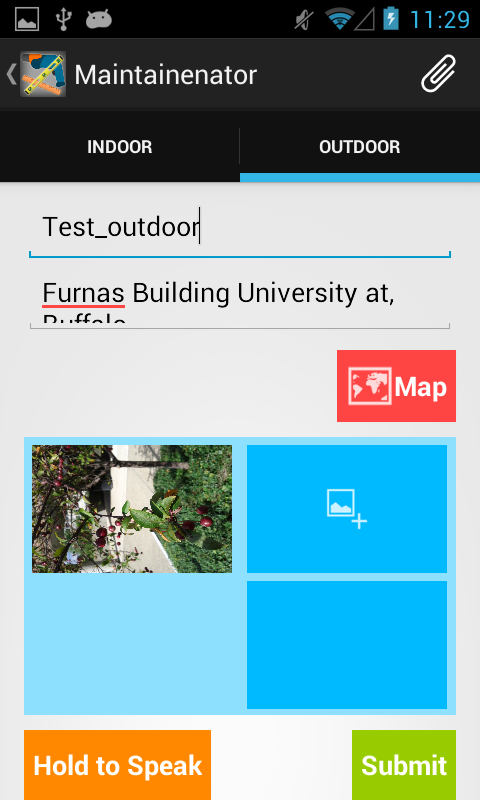
\includegraphics[scale=0.3]{images/outdoor_form.png}}
 \subfigure{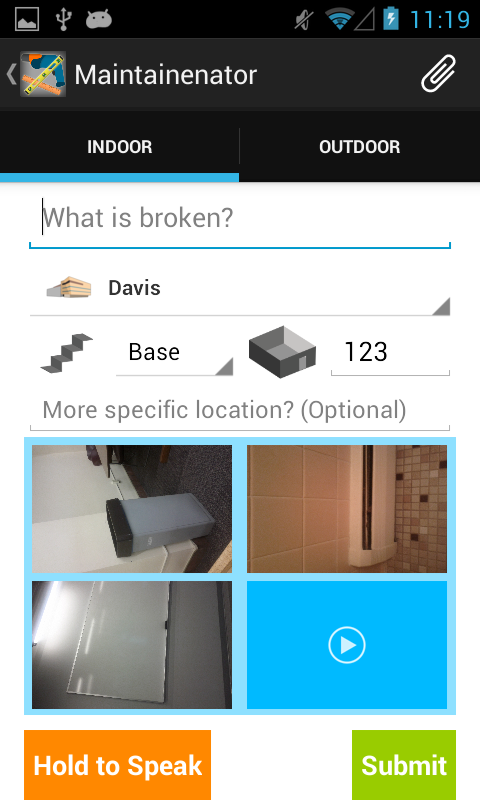
\includegraphics[scale=0.3]{images/indoor_form.png}}
 \caption{Issue form.} \label{fig:form}
 \end{figure*}
 The app requires submitter to at least provide a description, the location (which maybe acquired automatically as described in 
 Sec.~\ref{sec:localization} or replaced by submitter). For current indoor experiment, we only support four halls - Davis Hall, Jarvis Hall, 
 Furnas Hall and Ketter Hall.

Only text may not be that descriptive when describing an issue, thus we allow submitter to add photos and 
also an audio recording regarding the location or issue detail. By \texttt{long-press} the image area, 
the submitter can add up to three photos either from camera capture or gallery. Of course the submitter can view the full-size photo by
~\texttt{clicking} it and decide whether to keep it or replace it with a new one. Also, when submitter \texttt{holding} the recording button,
the app will recording the audio in \texttt{wav} format. We choose \texttt{wav} because it is the quick and dirty way to enable the recorded
audio can be played back both on Android and browser. The supported recording formats on Android (or to our best knowledge on Nexus S)
, e.g., \texttt{mp4}, \texttt{3gp} are not supported by current browsers. While the other formats supported by browser without any plugins,
\texttt{mp3, ogg} need third-party native libraries to be recorded on Android devices. 

\subsubsection{Others}
We will also save all the issues reported by one submitter locally on the Android device if the submitter choose to. Submitter can later
view the details of all the issues she reported before.

\subsection{Web Application}
For backend web service, we host our web application code on \texttt{heroku}~\footnote{\url{https://www.heroku.com/}}, which is a
cloud application platform that saves us from all kinds of pitfalls in servers management, deployment. 
Since \texttt{heroku} does not store static files as well as users upload files, 
we use \texttt{Amazon S3}~\footnote{\url{https://aws.amazon.com/s3/}} for this task.

We use \texttt{django}~\cite{django} web framework for our web application, its active community makes it much easier to develop web apps 
with numerous open source modules 
(a full list of all open source modules we used~\footnote{\url{https://github.com/forkloop/Maintainenator-backend/blob/master/requirements.txt}}). 
Our web application mainly has two components, private admin site, which is for maintainers to
manage all the reported issues, and public site, which is for every one to view existing reported issues.

\subsubsection{Private admin site}
\texttt{django} is already packed with an admin module, which is not that fancy. 
We instead use \texttt{grappelli}~\footnote{\url{http://www.grappelliproject.com/}} for polishing up the admin
interface. The admin site allow multiple maintainers to manage the reported issues, filtering them based on the location, severity level, status,
submitted date \textit{etc}. Maintainers can view the issues locations on Google Maps, get an idea of what the issues are via submitted photos and
audio recording. Maintainers can also record their working progress for a specific issue. 

\subsubsection{Public site}
The public site is intended for all to browse existing issues. We work on this public site to make it like an Single-page application~\cite{wiki-spa}, 
which can provide user a better experience with waterfall-like scrolling, no more page reloading when view different issues. 
We use \texttt{Backbone.js}~\footnote{\url{http://backbonejs.org/}} as for our frontend MVC. The whole interaction with the backend is via the 
RESTful JSON interface. 

\subsubsection{Others}
The web application provides a RESTful API, which the Android application uses to submit an issue, or the public site uses to retrieve the issues
information. We use \texttt{tastypie}~\footnote{\url{http://tastypieapi.org/}} to build this REST-style interface. We did little hack on \texttt{tastypie}
for this API to support file upload via \texttt{mixin}.

There are two kinds of processes for our web application, the \texttt{web process} is for responding all HTTP requests, either rendering a view or
return some JSON data. While the \texttt{worker process} is for all other not emergent tasks, \textit{e.g.}, sending submitters emails.

%==========
% CONCLUSION
%==========
\section{Conclusions}
\ldots


%==========
% ACKNOWLEDGE
%==========
\section{Acknowledgments}
\ldots

\bibliographystyle{abbrv}
\bibliography{sigproc}
\balancecolumns
% That's all folks!
\end{document}
